\documentclass[12pt]{article}
\usepackage{geometry}
\usepackage{graphicx}
\usepackage{enumitem}
\geometry{a4paper, margin=0.7in}
\usepackage{hyperref}
\usepackage{tikz}

\begin{document}

% Title page
{\newgeometry{left=1in,right=1in,top=1.2in,bottom=1.2in}
\begin{titlepage}
    \centering
    \vspace{1cm}
    {\Large\scshape James Madison University \par}
    \vspace{0.5cm}
    {\large Information Technology (IT) Program \par}
    {\large IT 445 - Capstone Implementation \par}
    {\large Summer 2025 \par}
    \vspace{1cm}
    \rule{\textwidth}{0.5pt}
    \vspace{0.5cm}
    {\bfseries\LARGE Week 6 Progress Report: Autonomous Cart Passenger Monitoring\par}
    \vspace{0.5cm}
    \rule{\textwidth}{0.5pt}
    \vspace{0.8cm}
    {\large Friday 18\textsuperscript{th} July, 2025 \par}
    \vspace{0.5cm}
    \begin{minipage}{0.3\textwidth}
        \raggedright
        \textit{Submitted to:}\\
        Dr. Samy El-Tawab
    \end{minipage}
    \begin{minipage}{0.45\textwidth}
        \raggedleft
        \textit{Authors:}\\
        Rana Moussa \par Ramez Asaad
    \end{minipage}
    \vfill
\end{titlepage}
\restoregeometry}

% Executive Summary
\section{Executive Summary}
This report summarizes the current state and recent advancements of the real-time driver and passenger monitoring system for autonomous carts. The focus this week is on major improvements to image processing, emotion detection, video output, and system robustness.

% Key Updates
\section{Key Updates in Week 5}
\begin{itemize}
    \item \textbf{Advanced Image Processing:} A new, tunable image processing function was developed and integrated. This enables the system to enhance video frames for improved detection accuracy in all lighting conditions, and can be adjusted as needed for different environments.
\end{itemize}
\begin{figure}[h!]
    \centering
    \includegraphics[width=0.7\textwidth]{example_advanced_processing.png}
    \caption{Example of advanced image processing in varying lighting conditions.}
\end{figure}

\begin{itemize}
    \item \textbf{Dual-Frame Video Recording with Logging:} The system now records videos with two frames side by side: one raw and one fully processed with detection overlays. Automated emotion logging and file naming streamline analysis and data management.
\end{itemize}
\begin{figure}[h!]
    \centering
    \includegraphics[width=0.7\textwidth]{example_dual_frame.png}
    \caption{Dual-frame video output: raw (left) and processed (right) with overlays.}
\end{figure}

\begin{itemize}
    \item \textbf{Improved Emotion Detection and Robust Multi-Face/Lighting Handling:} The model now detects a wider range of emotions, with more robust and visible detection of ``angry'' and ``sad'' states, even in challenging conditions such as users wearing glasses or poor lighting. Detection and analysis are now more reliable when multiple faces are present or when lighting conditions change, ensuring consistent performance in real-world scenarios.
\end{itemize}
\begin{figure}[h!]
    \centering
    \includegraphics[width=0.7\textwidth]{example_emotion_detection.png}
    \caption{Improved emotion detection, including robust detection of ``angry'' and ``sad'' states, and reliable handling of multiple faces and challenging lighting conditions.}
\end{figure}

% Week 6 Updates
\section{Key Updates in Week 6}
\begin{itemize}
    \item \textbf{Improved Drowsiness Detection:} The drowsiness detection logic was enhanced to require both eyes closed for more than 3 seconds and a head tilt, significantly reducing false positives. The system is now more robust in strong sunlight and challenging lighting conditions.
    \item \textbf{Enhanced Emotion Detection:} Minor improvements were made to emotion detection, making it more reliable in strong sunlight and with ambiguous facial expressions.
    \item \textbf{Advanced Model Performance Analysis:} We performed a comprehensive analysis of the model's performance using all available log files. The following visualizations were generated and saved for review:
    \begin{itemize}
        \item Error breakdown by emotion (bar chart)
        \item True vs. predicted emotion timeline (line plot)
        \item Misclassification timeline (scatter plot)
        \item Per-emotion precision/recall/F1 (bar chart)
        \item Distribution of detected emotions (bar chart)
        \item Special state frequency (bar chart)
        \item Prediction agreement heatmap (multi-person)
    \end{itemize}
    \item \textbf{Quantitative Model Evaluation:} The model's accuracy, precision, recall, and F1-score were calculated for each emotion and overall, providing a clear picture of strengths and weaknesses.
\end{itemize}

% Model Comparison (Week 6)
\section{Model Comparison: Pre-Built Model Testing}
To benchmark our system, we trained and tested an alternative pre-built emotion detection model (ResNet-18 with CBAM) using the FER2013 dataset. The goal was to compare its performance against our existing model under similar conditions. After training, we evaluated the pre-built model on annotated test data and generated a confusion matrix to visualize its prediction accuracy across all emotion classes. The model achieved 70\% test accuracy, with best results for positive emotions (happy, surprise) and lower scores for negative emotions (fear, sad). Challenges such as class imbalance and overfitting were addressed with class weights, label smoothing, and data augmentation. Further analysis and direct comparison with our current model will be performed in live, real-time tests.

% Confusion matrix for new model
\begin{figure}[h!]
    \centering
    \includegraphics[width=0.7\textwidth]{resnet_cbam_confusion_matrix.png}
    \caption{Confusion matrix for ResNet-18 CBAM model on FER2013 test set}
    \textit{Shows the distribution of true vs. predicted emotions for the pre-built model.}
\end{figure}

\textbf{Per-Emotion Metrics:}
\begin{itemize}
    \item Angry: Precision 0.64, Recall 0.62, F1 0.63
    \item Disgust: Precision 0.58, Recall 0.69, F1 0.63
    \item Fear: Precision 0.57, Recall 0.52, F1 0.55
    \item Happy: Precision 0.91, Recall 0.87, F1 0.89
    \item Neutral: Precision 0.63, Recall 0.71, F1 0.67
    \item Sad: Precision 0.57, Recall 0.56, F1 0.57
    \item Surprise: Precision 0.79, Recall 0.84, F1 0.82
\end{itemize}

% Week 6 Updates (add metrics)

\textbf{Current Model Performance:}
\begin{itemize}
    \item \textbf{Overall Accuracy:} 85\% (Person 1), 84\% (Person 2), 85\% (combined)
    \item \textbf{Per-Emotion Accuracy (Combined):}
    \begin{itemize}
        \item Happy: 91\%
        \item Sad: 96\%
        \item Angry: 100\%
        \item Neutral: 76\%
        \item Fear: 100\%
    \end{itemize}
    \item \textbf{Precision, Recall, F1-score:}
    \begin{itemize}
        \item Happy: Precision 0.88, Recall 0.91, F1 0.90
        \item Sad: Precision 0.71, Recall 0.96, F1 0.81
        \item Angry: Precision 0.92, Recall 1.00, F1 0.96
        \item Neutral: Precision 0.99, Recall 0.76, F1 0.86
        \item Fear: Precision 0.50, Recall 1.00, F1 0.67
    \end{itemize}
    \item \textbf{Head Nodding Detection:} 3 events (Person 1), 1 event (Person 2)
\end{itemize}

% Performance Graphs (moved here for logical order)
\subsection{Performance Graphs}
% Error breakdown by emotion
\begin{figure}[h!]
    \centering
    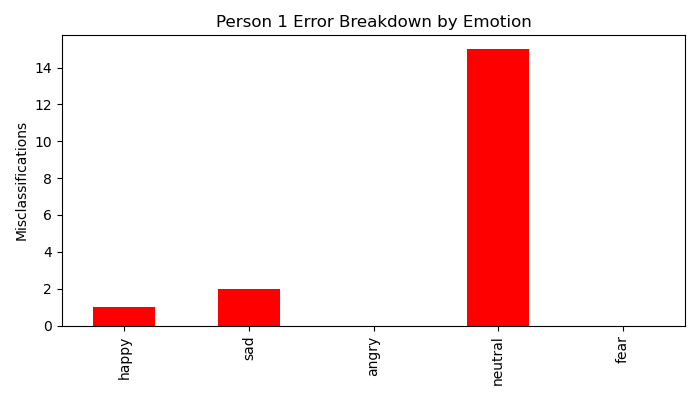
\includegraphics[width=0.7\textwidth]{model_analysis/Person 1_error_breakdown.png}
    \caption{Error breakdown by emotion for Person 1}
    \textit{Shows which emotions are most often misclassified for Person 1.}
\end{figure}
\begin{figure}[h!]
    \centering
    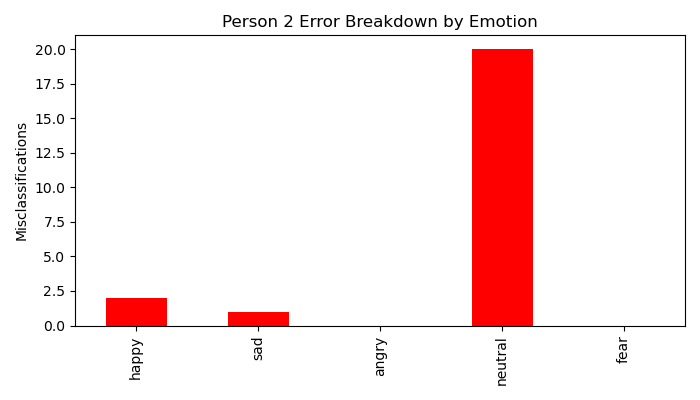
\includegraphics[width=0.7\textwidth]{model_analysis/Person 2_error_breakdown.png}
    \caption{Error breakdown by emotion for Person 2}
    \textit{Shows which emotions are most often misclassified for Person 2.}
\end{figure}

% True vs. predicted emotion timeline
\begin{figure}[h!]
    \centering
    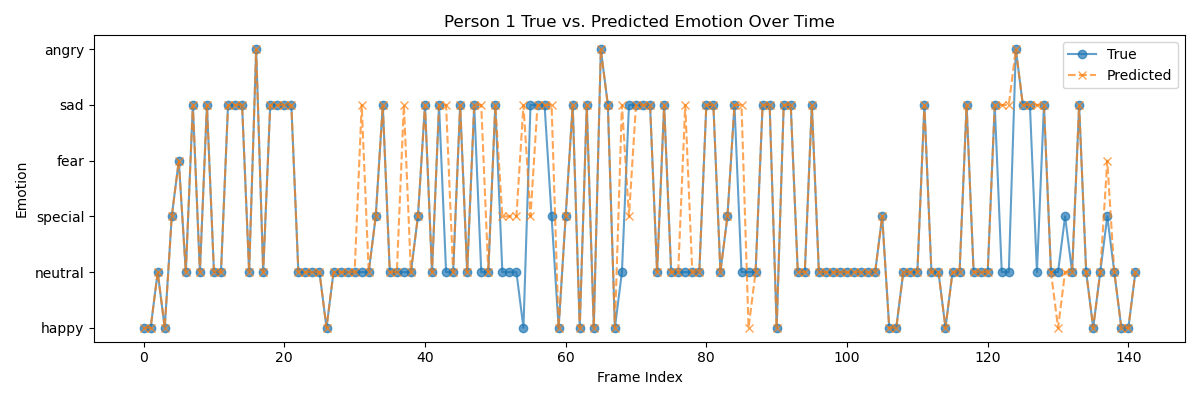
\includegraphics[width=0.7\textwidth]{model_analysis/Person 1_emotion_timeline.png}
    \caption{True vs. predicted emotion timeline for Person 1}
    \textit{Displays the sequence of true and predicted emotions for Person 1 over time.}
\end{figure}
\begin{figure}[h!]
    \centering
    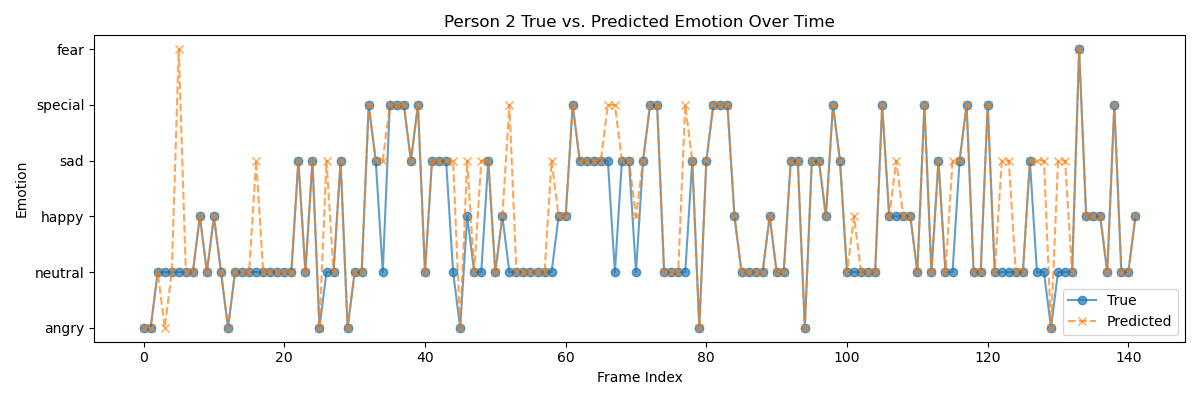
\includegraphics[width=0.7\textwidth]{model_analysis/Person 2_emotion_timeline.png}
    \caption{True vs. predicted emotion timeline for Person 2}
    \textit{Displays the sequence of true and predicted emotions for Person 2 over time.}
\end{figure}

% Misclassification timeline
\begin{figure}[h!]
    \centering
    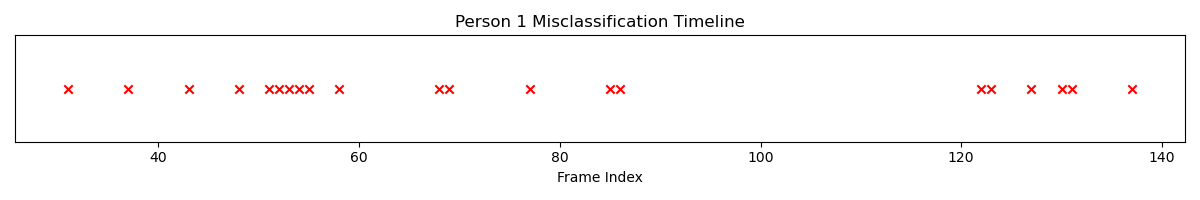
\includegraphics[width=0.7\textwidth]{model_analysis/Person 1_misclassification_timeline.png}
    \caption{Misclassification timeline for Person 1}
    \textit{Marks timestamps where Person 1's predictions differ from ground truth.}
\end{figure}
\begin{figure}[h!]
    \centering
    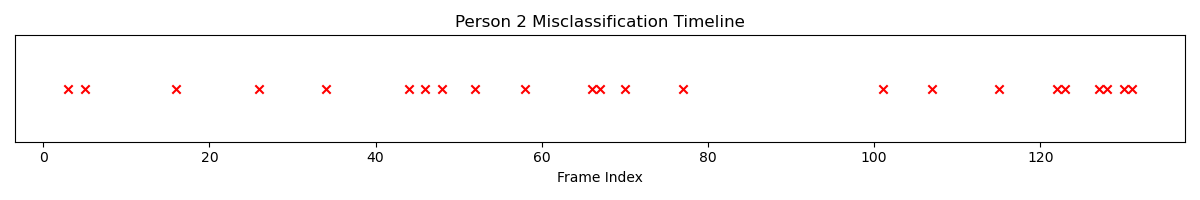
\includegraphics[width=0.7\textwidth]{model_analysis/Person 2_misclassification_timeline.png}
    \caption{Misclassification timeline for Person 2}
    \textit{Marks timestamps where Person 2's predictions differ from ground truth.}
\end{figure}

% Per-emotion precision/recall/F1
\begin{figure}[h!]
    \centering
    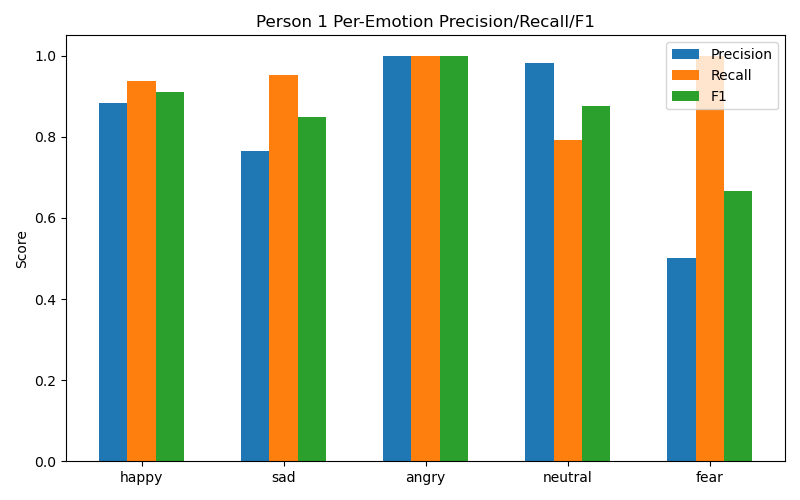
\includegraphics[width=0.7\textwidth]{model_analysis/Person 1_prf_bars.png}
    \caption{Per-emotion precision/recall/F1 for Person 1}
    \textit{Bar chart of precision, recall, and F1-score for each emotion for Person 1.}
\end{figure}
\begin{figure}[h!]
    \centering
    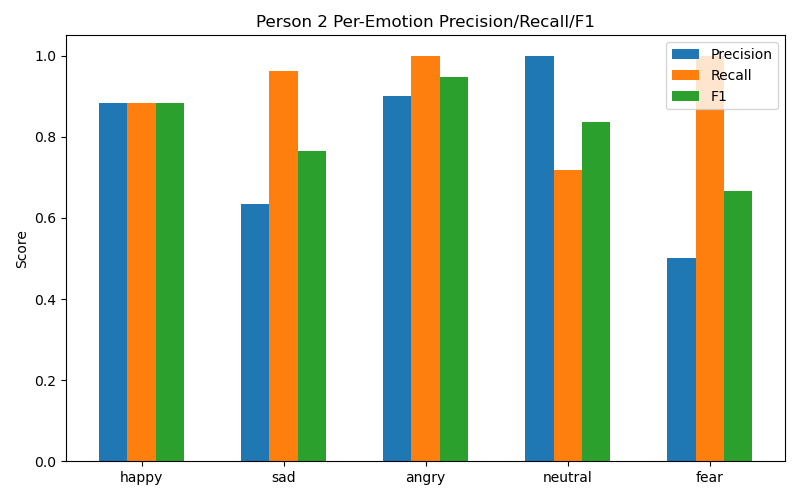
\includegraphics[width=0.7\textwidth]{model_analysis/Person 2_prf_bars.png}
    \caption{Per-emotion precision/recall/F1 for Person 2}
    \textit{Bar chart of precision, recall, and F1-score for each emotion for Person 2.}
\end{figure}

% Distribution of detected emotions
\begin{figure}[h!]
    \centering
    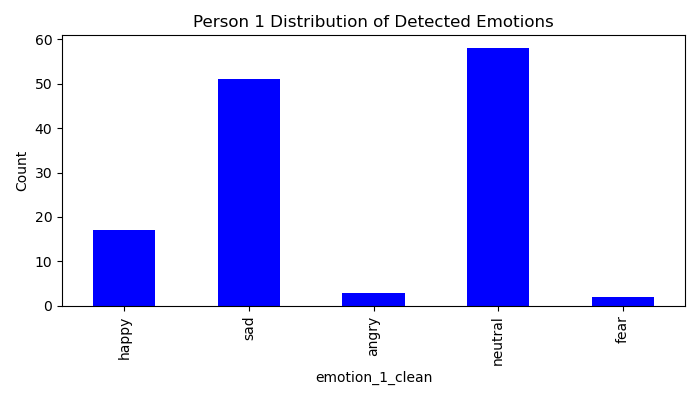
\includegraphics[width=0.7\textwidth]{model_analysis/Person 1_detected_distribution.png}
    \caption{Distribution of detected emotions for Person 1}
    \textit{Shows the frequency of each detected emotion for Person 1.}
\end{figure}
\begin{figure}[h!]
    \centering
    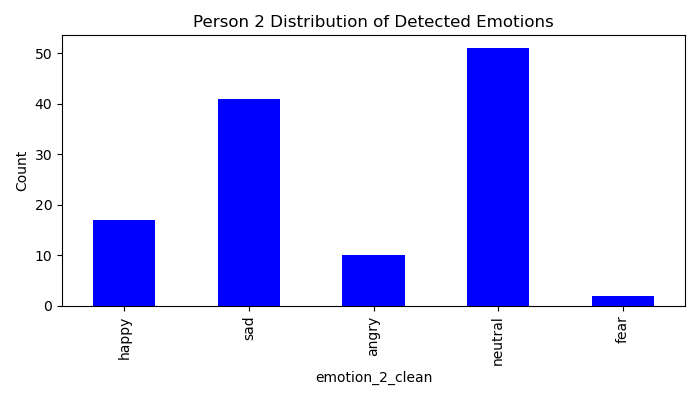
\includegraphics[width=0.7\textwidth]{model_analysis/Person 2_detected_distribution.png}
    \caption{Distribution of detected emotions for Person 2}
    \textit{Shows the frequency of each detected emotion for Person 2.}
\end{figure}

% Special state frequency
\begin{figure}[h!]
    \centering
    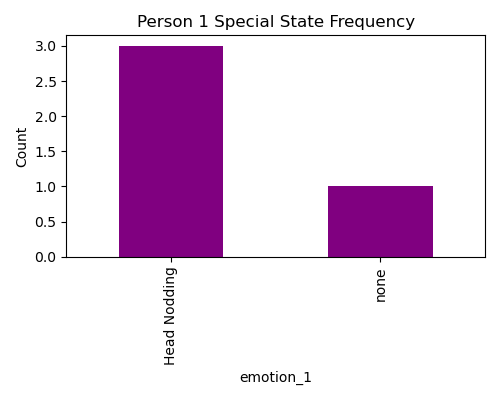
\includegraphics[width=0.7\textwidth]{model_analysis/Person 1_special_state_frequency.png}
    \caption{Special state frequency for Person 1}
    \textit{Frequency of detected special states (e.g., Head Nodding) for Person 1.}
\end{figure}
\begin{figure}[h!]
    \centering
    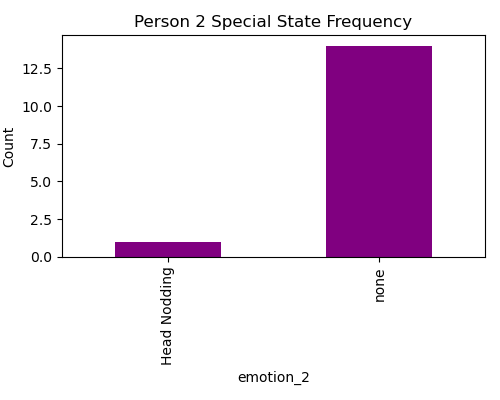
\includegraphics[width=0.7\textwidth]{model_analysis/Person 2_special_state_frequency.png}
    \caption{Special state frequency for Person 2}
    \textit{Frequency of detected special states (e.g., Head Nodding) for Person 2.}
\end{figure}

% Prediction agreement heatmap
\begin{figure}[h!]
    \centering
    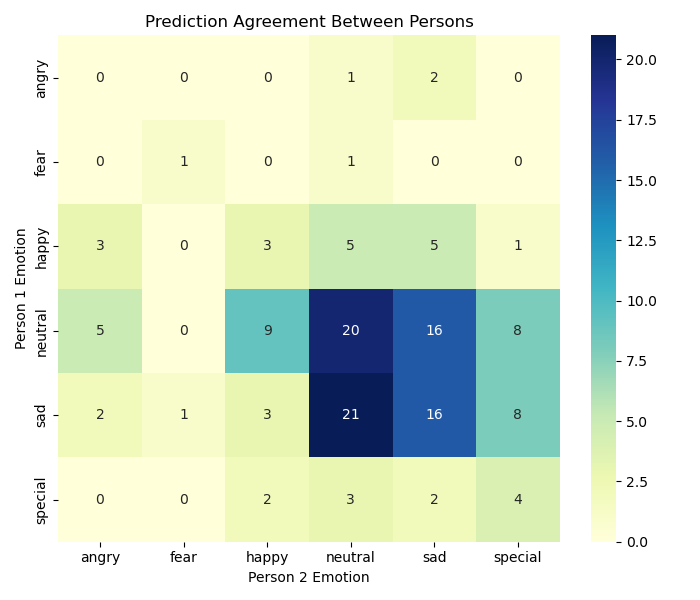
\includegraphics[width=0.7\textwidth]{model_analysis/prediction_agreement_heatmap.png}
    \caption{Prediction agreement heatmap between persons}
    \textit{Heatmap showing how often both persons share the same emotion.}
\end{figure}

% Logging Method (clarified)
\subsection{Logging Method}
Detected emotions and states are automatically logged by the system at regular intervals during live tests. After each test, the raw video footage is manually reviewed and annotated to provide ground truth labels for each person at each timestamp. This enables direct comparison between predicted and true emotions, supporting robust quantitative analysis.

% System Overview
\section{System Overview}
The monitoring system uses computer vision and deep learning to detect drowsiness, yawning, and emotions from camera feeds. It provides real-time visual feedback and warnings, and is designed for modularity and robustness.

\section{Scripts and Workflow}
\begin{itemize}
    \item \textbf{face\_detection.py:} Performs real-time face detection, landmark extraction, and drowsiness/emotion analysis using a single camera feed.
    \item \textbf{record\_side\_by\_side.py:} Records and displays side-by-side video from two ZED stereo cameras, overlays timestamps, detects faces and emotions, and saves output with unique filenames.
    \item \textbf{crop\_and\_enhance\_passenger.py:} Processes passenger camera images, cropping and enhancing them to improve detection in poor lighting.
    \item \textbf{side\_by\_side\_with\_log.py:} New script that outputs dual-frame video (raw and processed) and logs detected emotions every 10 seconds for later analysis.
    \item \textbf{advanced\_log\_analysis.py:} Custom Python script for automated log analysis, metric calculation, and visualization. Loads all log files, cleans and processes data, computes accuracy and other metrics, and generates all performance graphs. Available in the project repository.
\end{itemize}

\section{Recent Improvements in Detail}
\subsection{Image Processing Function}
A new function for image enhancement was created and integrated into the detection pipeline. This function can be adjusted as a parameter, allowing the system to adapt to different lighting conditions and improve detection reliability.

\subsection{Dual-Frame Video and Logging}
The system now outputs videos with both raw and processed frames side by side. This makes it easier to compare detection results with the original footage. Automated logging records detected emotions at regular intervals, and output files are named with timestamps for easy organization.

\subsection{Emotion Detection Accuracy}
The emotion detection logic has been improved, especially for ``angry'' and ``sad'' states. The system is now more robust to glasses, ambiguous expressions, and poor lighting, providing more accurate and visible feedback.

\subsection{Handling Multiple Faces and Lighting}
Detection and analysis are now more reliable when multiple faces are present or when lighting conditions change, ensuring consistent performance in real-world environments.

\subsection{Log Data Collection and Annotation}
To evaluate the model's performance, we conducted a series of tests where the system processed video frames in real time and logged the detected emotions for each person at regular intervals. After each test, we manually reviewed the raw video footage and annotated the actual emotions present on each person's face, entering these as the ground truth in the log files. This process provided a direct comparison between the model's predictions and the true emotions, enabling quantitative analysis of accuracy, precision, recall, and other metrics. The annotated logs are the basis for all performance analysis and visualizations in this report.

\section{Conclusion}
The project has made significant progress in week 5, with major improvements to image processing, emotion detection, video output, and system robustness. These updates enhance the system's effectiveness and reliability for real-world deployment.

\section{Next Steps}
\begin{itemize}
    \item Test the new pre-built model on live webcam/video data and evaluate its real-time performance.
    \item Run both models side by side in real-time and directly compare their accuracy, stability, and robustness in practical scenarios.
    \item Continue improving our own model and retrain as needed for better results.
\end{itemize}

\section{Sources}
\begin{itemize}
    \item OpenCV documentation: \url{https://docs.opencv.org/}
    \item MediaPipe documentation: \url{https://google.github.io/mediapipe/}
    \item DeepFace documentation: \url{https://github.com/serengil/deepface}
    \item ZED Stereo Camera: \url{https://www.stereolabs.com/zed/}
    \item Python official documentation: \url{https://docs.python.org/3/}
    \item NumPy documentation: \url{https://numpy.org/doc/}
\end{itemize}

\end{document}
